\documentclass[conference,pdf,table,xcdraw, utf8]{IEEEtran}
\IEEEoverridecommandlockouts

\usepackage[T1]{fontenc} 
\usepackage{cite}
\usepackage{amsmath,amssymb,amsfonts}
\usepackage{algorithmicx}
\usepackage{graphicx}
\usepackage{textcomp}
\usepackage{xcolor}
\usepackage{listings}
\usepackage{changepage} 
\usepackage{float}
\usepackage{inputenc}
\usepackage{xcolor}
\usepackage{listings}
\usepackage{algorithm}
\usepackage{graphics,graphicx}
\usepackage{pstricks,pst-node,pst-tree}
\usepackage{listings}
\usepackage{color}
\usepackage{algpseudocode}
\usepackage{enumerate}
\usepackage{url}
\usepackage{relsize}
\usepackage{contour}
\usepackage{pstricks}

\def\UrlBreaks{\do\/\do-}

\lstset{basicstyle=\ttfamily,columns=fullflexible}

\definecolor{mediumgray}{rgb}{0.3, 0.4, 0.4}
\definecolor{mediumblue}{rgb}{0.0, 0.0, 0.8}
\definecolor{forestgreen}{rgb}{0.13, 0.55, 0.13}
\definecolor{darkviolet}{rgb}{0.58, 0.0, 0.83}
\definecolor{royalblue}{rgb}{0.25, 0.41, 0.88}
\definecolor{lightgreen}{rgb}{0.21, 0.62, 0.54}

\lstdefinelanguage{JavaScript}{
  morekeywords=[1]{async, break, continue, delete, function, in, new, this, typeof, var, while, with, let, const, enum, extends, finally, from, implements, import, instanceof, false, true, null, Infinity},
  % Literals, primitive types, and reference types.
  morekeywords=[2]{void, undefined, boolean, number, string, Array, Boolean, Date, Math, Number, String, Object},
  % Built-ins.
  morekeywords=[3]{if, else, for, export, import, default, return, await},
  sensitive,
  morecomment=[s]{/*}{*/},
  morecomment=[l]//,
  morecomment=[s]{/**}{*/}, % JavaDoc style comments
  morestring=[b]',
  morestring=[b]"
  morestring=[b]` % Interpolation strings.
}[keywords, comments, strings]

\lstdefinelanguage[TypeScript]{JavaScript}[]{JavaScript}{
    morekeywords=[2]{Move, State},
    morekeywords=[4]{Cell},
}

\lstalias[]{TS}[TypeScript]{JavaScript}

\lstdefinestyle{javascriptbase} {%
  basicstyle={\footnotesize\ttfamily},   
  frame=b,
  % line-numbers
  xleftmargin={0.75cm},
  numbers=left,
  stepnumber=1,
  firstnumber=1,
  numberfirstline=true,	
  % Code design
  identifierstyle=\color{black},
  keywordstyle=\color{mediumblue},
  keywordstyle={[2]\color{lightgreen}},
  keywordstyle={[3]\color{darkviolet}},
  stringstyle=\color{brown}\ttfamily,
  commentstyle=\color{green}\ttfamily,
  % Code
  alsodigit={.:;},	
  tabsize=2,
  showtabs=false,
  showspaces=false,
  showstringspaces=false,
  extendedchars=true,
  breaklines=true,
}

\lstdefinestyle{javascript}{
  language=JavaScript,
  style=javascriptbase,
}

\lstdefinestyle{ts}{
  language=TS,
  style=javascriptbase,
  keywordstyle={[4]\color{lightgreen}},
}

\lstdefinestyle{typescript}{
  language=TypeScript,
  style=javascriptbase,
  keywordstyle={[4]\color{lightgreen}},
}

\begin{document}
%\BeforeBeginEnvironment{minted}{\begin{tcolorbox}}
%\AfterEndEnvironment{minted}{\end{tcolorbox}}
\newcommand{\subtitlerelsize}{1}
\newcommand{\subtitlelinesep}{0.2em}

\title{MinMax\\[\subtitlelinesep]%
    \smaller[\subtitlerelsize]{}Game Theory}
\author{\IEEEauthorblockN{1\textsuperscript{st} Ikic}
    \IEEEauthorblockA{\textit{Mobile Computing} \\
        \textit{FH OÖ Campus Hagenberg}\\
        Hagenberg, Austria \\
        S2010237031@fhooe.at
    }
    \and
    \IEEEauthorblockN{2\textsuperscript{nd} Shehata}
    \IEEEauthorblockA{\textit{Mobile Computing} \\
        \textit{FH OÖ Campus Hagenberg}\\
        Hagenberg, Austria \\
        S2010237022@fhooe.at
    }
    \and
    \IEEEauthorblockN{3\textsuperscript{rd} Milosavljevic}
    \IEEEauthorblockA{\textit{Mobile Computing} \\
        \textit{FH OÖ Campus Hagenberg}\\
        Hagenberg, Austria \\
        S2010237014@fhooe.at
    }
}

\maketitle

\begin{abstract}

    Game theory belongs to the branch of applied mathematics, but is also used in philosophy, life science and social science. Game theory tries to mathematically explain the results of one person, depending on the result or action of another person. One of the most important results was formulated in 1928 by the mathematician John von Neumann and is called the Minimax Theorem. This theorem forms the basis for all subsequent findings in this field.

\end{abstract}

%%%%%%%%%%%%%%%%%%%%%%%%%%%%%%%%%%%%
%\clearpage
%%%%%%%%%%%%%%%%%%%%%%%%%%%%%%%%%%%%

%\tableofcontents

%%%%%%%%%%%%%%%%%%%%%%%%%%%%%%%%%%%%
%\clearpage
%%%%%%%%%%%%%%%%%%%%%%%%%%%%%%%%%%%%


\section{Introduction}
The MiniMax theorem is about finding the optimal game strategy for finite two-person zero-sum games with perfect infromation. With small modifications, it can be used in games such as Go, Chess, Checkers, Four-in-a-row and Tic-Tac-Toe. The MiniMax theorem forms the core of chess programs and chess computers. In 1996, the reigning world chess champion Garry Kasparov was only beaten by brute force calculations. In summary, the basic idea behind the Minimax algorithm is: "If I make this move, my opponent can only make these moves".~\cite{introduction}


\section{MiniMax Algorithm}
\subsection{Applying MiniMax Algorithm to Connect 4}
Here we will explain how the Minimax algorithm works, using the game Connect 4, as you can see in Figure \ref{figure:connect4}, as an example.

\begin{figure}[H]
    \centering
    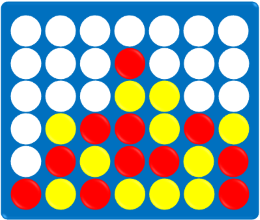
\includegraphics[scale=0.65]{images/connect4.png}
    \caption{Connect 4}
    \label{figure:connect4}
\end{figure}

%Kurz erklärt wie 4 Gewinnt funktioniert
\subsection{Connect 4 rules of the game}
Connect-Four may be a game for two persons. Both players have 21 indistinguishable pieces. Within the standard frame of the game, one set of pieces is yellow and the other set is red. The game is played on a vertical, rectangular board comprising of 7 vertical columns of 6 squares each. If a piece is put in one of the columns, it'll drop down to the last empty square within the column. As soon as a column contains 6 pieces, no other piece can be put within the column. Putting a piece in one of the columns is called: a move. The players make their moves in turn.~\cite{4connect_rules2}

Try to get four pieces of your colour into a horizontal, vertical or diagonal row before your opponent! It is not only important to pay attention to your own success, but also to ensure that your opponent does not succeed in completing the row. If all 42 pieces are played and no player has achieved this goal, the game will end in a draw.~\cite{4connect_rules}

Figure \ref{figure:4gewinnt_white_wins.PNG} shows positions in which White has won the game:

\begin{figure}[H]
    \centering
    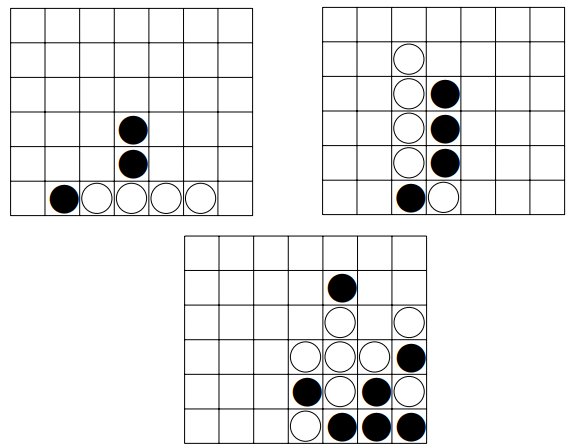
\includegraphics[scale=0.85]{images/4gewinnt_white_wins.PNG}
    \caption{White has won}
    \label{figure:4gewinnt_white_wins.PNG}
\end{figure}

A possible draw position is shown in Figure \ref{figure:4gewinnt_draw.PNG}

\begin{figure}[H]
    \centering
    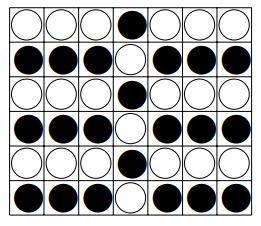
\includegraphics[scale=0.95]{images/4gewinnt_draw.PNG}
    \caption{White has won}
    \label{figure:4gewinnt_draw.PNG}
\end{figure}

\subsection{Mini-Max algorithm and Connect 4}
The MinMax algorithm belongs to the backtracking algorithms and can be used in several ways. Basically, it is used in decision and game theory, where it will try to find the optimal move. It is always assumed that our opponent will also choose the optimal move against us. In the MinMax algorithm there are two players. One is called the maximiser and the other one is called the minimiser. The minimiser will try to achieve the lowest score and the maximiser will try to do exactly the opposite. With each move, the state of the board changes. Each board state is therefore assigned a certain value. If the maximiser has the advantage in a certain state in the game, the score of the board will tend to be positive. Conversely, if the minimiser has the advantage in the game at the same state, the value will tend to be negative.~\cite{MinMaxConnect4}

\begin{table}[H]
    \begin{tabular}{|l|l|}
        \hline
        \multicolumn{1}{|c|}{\textbf{Minimax tree notion}} & \multicolumn{1}{c|}{\textbf{Minimax game notion}}                                           \\ \hline
        Minimax tree                                       & \begin{tabular}[c]{@{}l@{}}All possible \\ board configurations\end{tabular}                \\ \hline
        Node in the tree                                   & Board configuration                                                                         \\ \hline
        Edge from a max node to a min node                 & \begin{tabular}[c]{@{}l@{}}Personal move \\ (move by player max)\end{tabular}               \\ \hline
        Edge from a min node to a max node                 & \begin{tabular}[c]{@{}l@{}}Adversary move \\ (move by player min)\end{tabular}              \\ \hline
        Node value                                         & \begin{tabular}[c]{@{}l@{}}Quality of a given \\ board position\end{tabular}                \\ \hline
        Leaf node                                          & \begin{tabular}[c]{@{}l@{}}Outcome of a game \\ (either win, tie or lose)\end{tabular}      \\ \hline
        Solution path                                      & \begin{tabular}[c]{@{}l@{}}Sequence of moves \\ leading to the best \\ outcome\end{tabular} \\ \hline
    \end{tabular}
    \caption{Relation between minimax trees and minimax games.}
    \label{table:1}
\end{table}

For our MinMax algorithm, a simple game tree would look like the one shown in figure ~\ref{figure:tree_step1.PNG}.~\cite{MinMaxConnect4}

\begin{figure}[H]
    \centering
    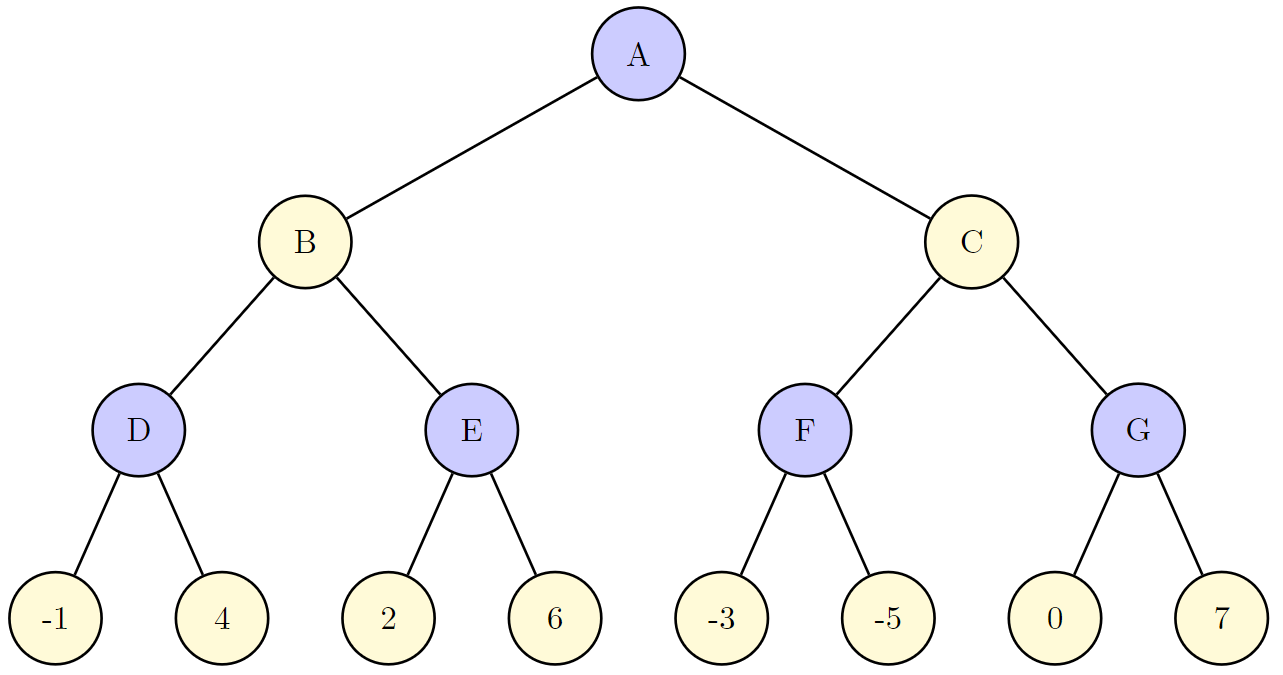
\includegraphics[scale=0.39]{images/tree_step1.PNG}
    \caption{Simple starting game tree}
    \label{figure:tree_step1.PNG}
\end{figure}

\subsubsection{MinMax explanation}
Our MinMax algorithm searches the entire depth of the game tree down to the leaf nodes. This search is also called a depth-first search (DFS). The next example will illustrate the algorithm.~\cite{MinMaxConnect4_2}

First, the algorithm generates the entire game tree and creates the utility values for the end states by applying the utility function as shown in figure 2. For example, in the figure 2 tree diagram, let us assume A as the initial state of the tree. Suppose the maximiser takes the first move, which in the worst case has an initial value equal to negative infinity. Then the minimiser takes the next move, which in the worst case has an initial value equal to positive infinity.

Next, we consider the maximiser with the initial value minus infinity. Each end node is compared with the maximiser's value and finally the maximum value is stored in each maximiser node. For example, let's take the third row (maximiser) from above.

\begin{itemize}
    \item for node D \contour{black}{$\longrightarrow max(max(-1,-\infty),4) = 4$}
    \item for node E \contour{black}{$\longrightarrow max(max(2,-\infty),6) = 6$}
    \item for node F \contour{black}{$\longrightarrow max(max(-3,-\infty),-5) = -3$}
    \item for node G \contour{black}{$\longrightarrow max(max(0,-\infty),7) = 7$}
\end{itemize}

Our tree now looks as shown in the following figure ~\ref{figure:tree_step2.PNG}.

\begin{figure}[H]
    \centering
    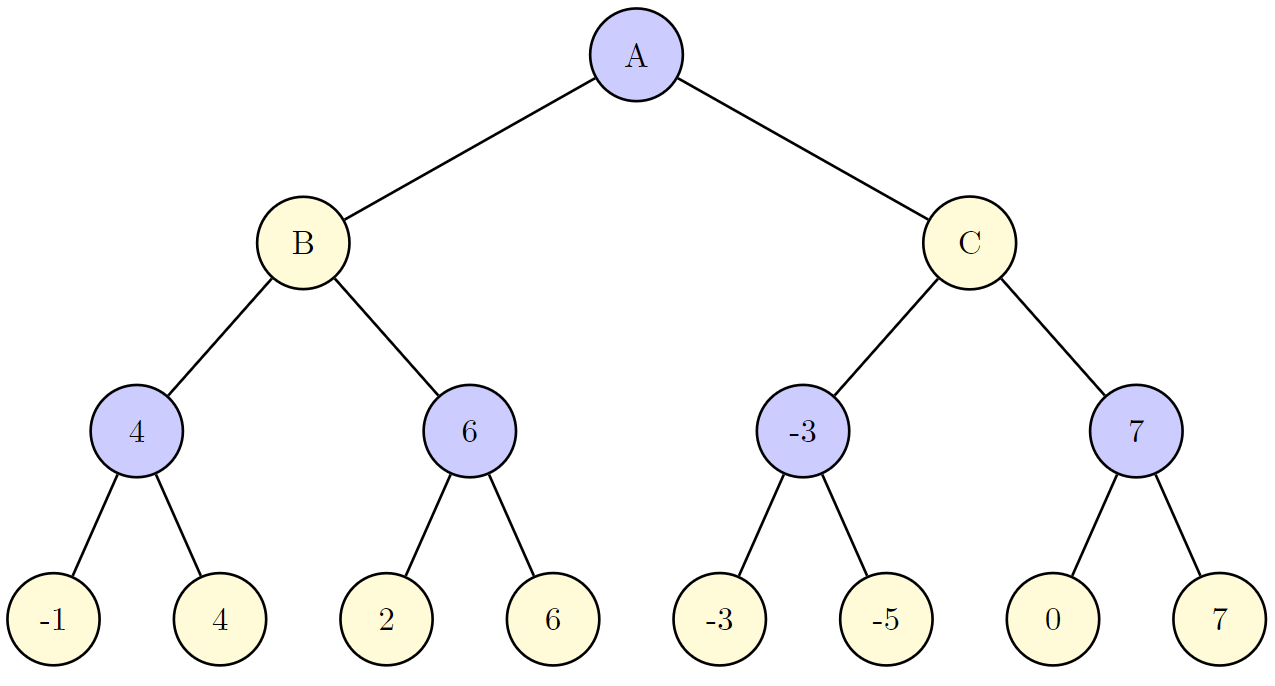
\includegraphics[scale=0.38]{images/tree_step2.PNG}
    \caption{MinMax game tree}
    \label{figure:tree_step2.PNG}
\end{figure}


We then compare the values of each node with the value of the minimiser, which is plus infinity.

\begin{itemize}
    \item for node B \contour{black}{$\longrightarrow min(min(4,+\infty),6) = 4$}
    \item for node C \contour{black}{$\longrightarrow min(min(-3,+\infty),7) = -3$}
\end{itemize}


Our tree now looks as shown in the following figure ~\ref{figure:tree_step3.PNG}.

\begin{figure}[H]
    \centering
    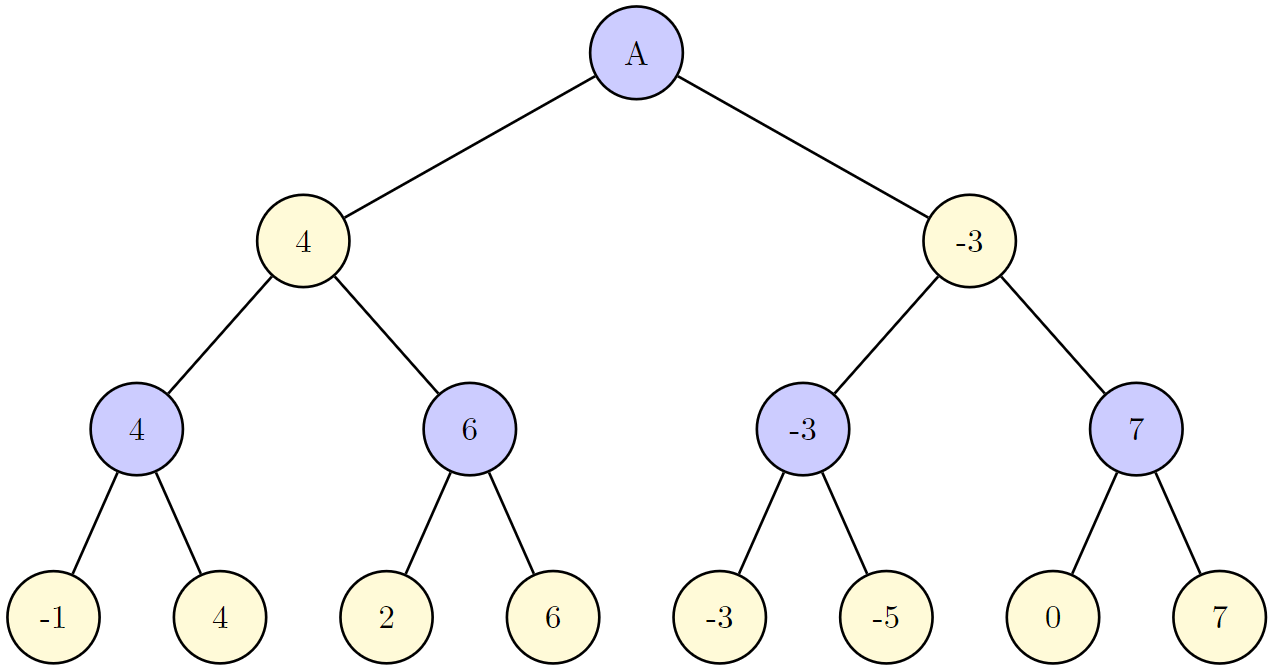
\includegraphics[scale=0.37]{images/tree_step3.PNG}
    \caption{MinMax game tree}
    \label{figure:tree_step3.PNG}
\end{figure}

Finally, the maximiser then chooses the maximum value between node B and node C again:

\begin{itemize}
    \item for node A \contour{black}{$\longrightarrow max(4,-3) = 4$}
\end{itemize}

This results in the following optimal gameplay also shown in figure \ref{figure:tree_final.PNG}:
A$\rightarrow$ B$\rightarrow$ D$\rightarrow$ I

\begin{figure}[H]
    \centering
    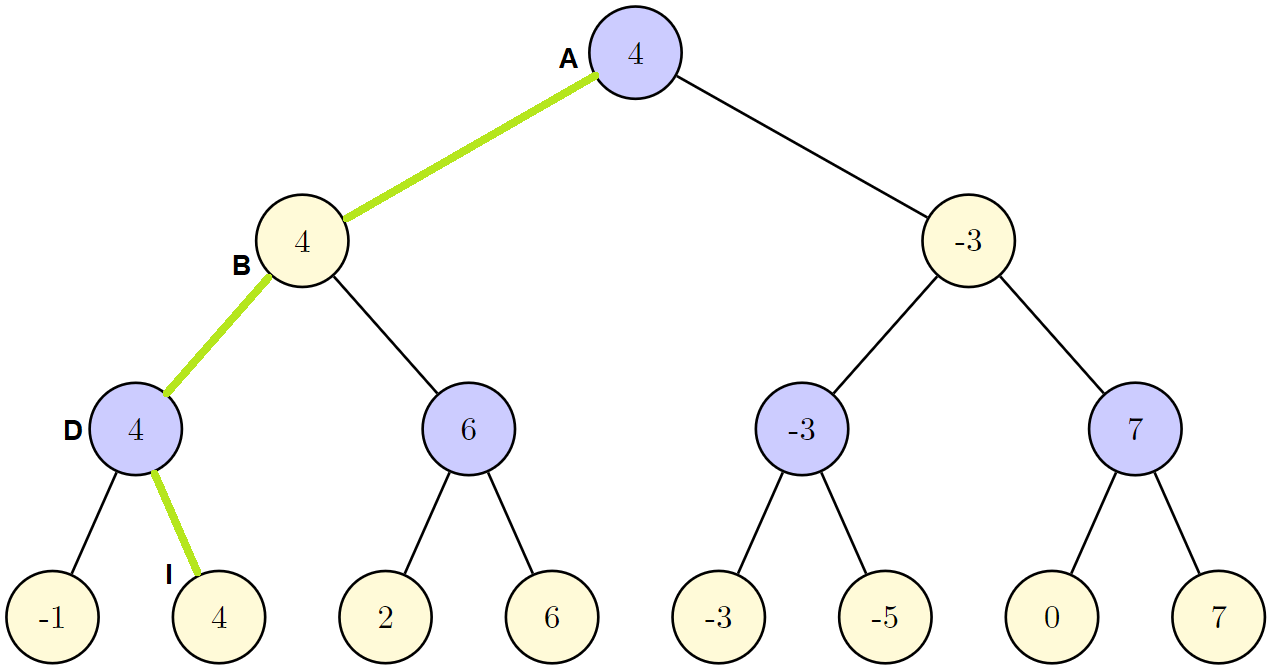
\includegraphics[scale=0.39]{images/tree_final.png}
    \caption{MinMax game tree}
    \label{figure:tree_final.PNG}
\end{figure}
\vspace{\fill}

\begin{lstlisting}[linewidth=\columnwidth,breaklines=true,mathescape=true,
caption=MinMax Pseudocode]
def minMax(node, depth, maximizingPlayer) is
  if depth = 0 or node is a terminal node then
    return the heuristic value of node
  if maximizingPlayer then
    value = -$\infty$
    for each child of node do
        value := max(value, minMax(child, depth - 1, FALSE))
    return value
  else (* minimizing player *)
    value = +$\infty$
    for each child of node do
        value := min(value, minMax(child, depth - 1, TRUE))
  return value
\end{lstlisting}

\begin{lstlisting}[style=ts,linewidth=\columnwidth,breaklines=true,
caption=MinMax Connect-4 source-code]
function minimax(state: State, depth = Infinity): Move | undefined {
	const player = state.player;

	const checkIsTerminal = (state: State, currentDepth: number): boolean =>
		currentDepth == 0 || state.utility !== 0 || state.moves.length === 0;

	const evalFn = (state: State): number =>
		player === Cell.PLAYER ? state.utility : -state.utility;

	function maximizer(state: State, depth: number): number {
		return getActions(state).reduce((prev, action) => {
			const [row, col] = action;
			const best = Math.max(prev, minimizer(result(state, action), depth - 1));
			state.board[row][col] = Cell.EMPTY;
			return best;
		}, -Infinity);
	}

	function minimizer(state: State, depth: number): number {
		return getActions(state).reduce((prev, action): number => {
			const [row, col] = action;
			const best = Math.min(prev, maximizer(result(state, action), depth - 1));
			state.board[row][col] = Cell.EMPTY;
			return best;
		}, Infinity);
	}
	
	let best = -Infinity;
	let bestMove: Move | undefined = undefined;

	for (const move of getActions(state)) {
		const [row, col] = move;
		const value = minimizer(result(state, move), depth - 1);
		state.board[row][col] = Cell.EMPTY;

		if (value > best) {
			best = value;
			bestMove = move;
		}
	}

	return bestMove;
}
\end{lstlisting}


\section{Optimization technique for MinMax}
\subsection{Alpha-Beta pruning}
One of the most practiced optimization techniques for the MinMax algorithm is alpha beta pruning. As an optimization technique it only adapts the MinMax algorithm's mechanism and can therefore not be regarded individually. \cite{nasa2018alpha} That is to say, the main purpose of this technique is speed enhancement whilst ensuring that no information loss occurs.
The Min-Max algorithm functions as a Depth first algorithm, starting on the left an traversing through the tree by always visiting the terminating leaf, where the pruning process takes place.
A node is being pruned from a tree or sub-tree if it is evident that the algorithm is not going to take that path. This optimizes runtime from $O(b^d)$to $O(b^d(d/2))$.


In order to further understand this technique it is necessary to look at the basic operations, which are depicted in the following example. The given MinMax tree uses blue nodes to symbolize the maximizing player and yellow for the minimizing player. Additionally the currently regarded node is colored orange and the already pruned nodes grey.

The tree traversal functions as previously explained in section 1. until the orange colored node is reached. There the tree evaluates if it is even necessary to further examine the underlying nodes.

\vspace{1em}
\newcommand{\Rect}[1]{ 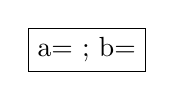
\begin{tikzpicture}
        \tikzset{byte/.append style={rectangle,
                    draw=black, fill=white,
                    minimum width=0.75cm,
                    minimum height=1cm,
                    anchor=north west,
                    align=center, font=\scriptsize}}
        \node[rectangle,draw] (r) at (0,0) {a= ; b= };
    \end{tikzpicture}}


\newcommand{\MaxNode}[1]{\Tcircle[fillstyle=solid,fillcolor=blue!20]{\makebox[2em] {#1}}}
\newcommand{\MinNode}[1]{\Tcircle[fillstyle=solid,fillcolor=yellow!20]{\makebox[2em] {#1}}}
\newcommand{\CurrentNode}[1]{\Tcircle[fillstyle=solid,fillcolor=orange!20]{\makebox[2em] {#1}}}
\newcommand{\PrunedNode}[1]{\Tcircle[fillstyle=solid,fillcolor=grey!20]{\makebox[2em] {#1}}}
\newcommand{\TestNode}[1]{
    \Tcircle[fillstyle=solid,fillcolor=grey!20]{
        \begin{tikzpicture}
            \draw (0,0) circle (2em);
            \draw (-2em,0) rectangle (2,0.5);
            \node[fillstyle=solid,fillcolor=grey!20]{{#1}}
        \end{tikzpicture}
    }
}

\begin{figure}[H]
    \centering
    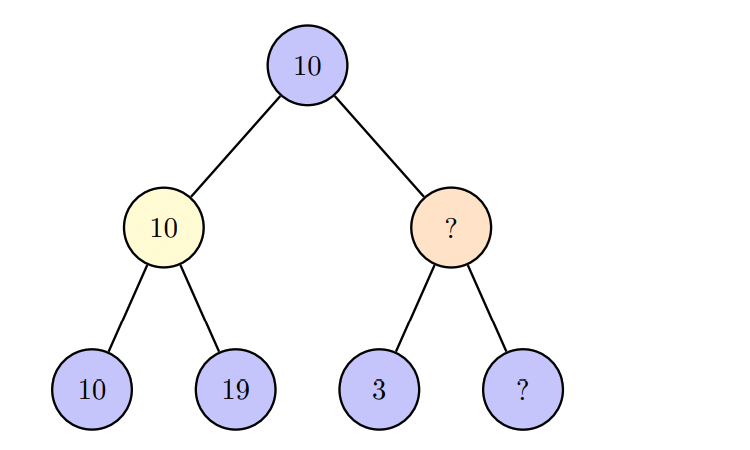
\includegraphics[scale=0.335]{images/pruning_tree1.png}
    \caption{Alpha-beta pruning}
    \label{figure:pruning1}
\end{figure}


%\pstree{\MaxNode{10}}
%   {\pstree{\MinNode{10}}
%        {\MaxNode{10}
%           \MaxNode{19}
%           }
%        \pstree{\CurrentNode{?}}
%              {\MaxNode{3}
%                    \MaxNode{?}}}
%    \vspace{1em} 

Since the minimizing player always chooses the lowest value it is evident that the orange marked node can only obtain a value  $\leq \ $3. Consequently it is clear that the root node will choose the highest value and therefore will not consider the right branch at all, since it will not provide a value higher than 10.

\begin{figure}[H]
    \centering
    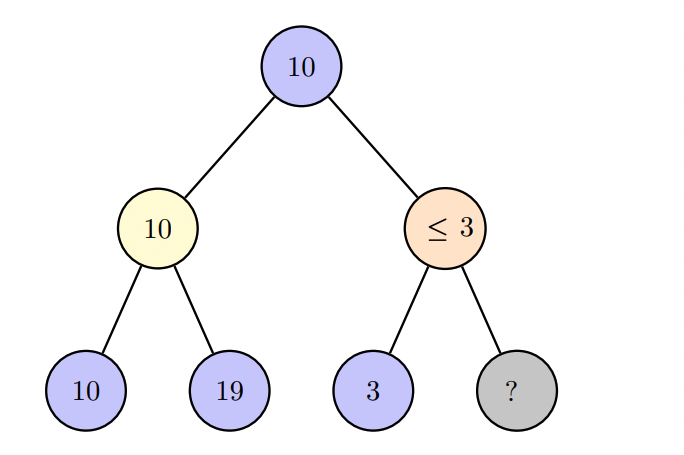
\includegraphics[scale=0.35]{images/pruning_tree2.png}
    \caption{Alpha-beta pruning}
    \label{figure:pruning2}
\end{figure}

%\vspace{1em} 
%\pstree{\MaxNode{10}}
%   {\pstree{\MinNode{10}}
%       {\MaxNode{10}
%         \MaxNode {19}
%         
%          }
%      \pstree{\CurrentNode{ $\leq \ $3}}
%            { \MaxNode{3}
%                   \PrunedNode{? }}}
%  \vspace{1em} 

Although pruning evidently shortens the amount of time needed to traverse the tree, it is nonetheless not guaranteed to occur. This becomes clear when switching the leaf node 3 with for instance the value 30. In that case no sub-tree or nodes could have been pruned. This leads to the conclusion that pruning depends on the moves order. Ideally the moves are ordered from best to worst.

%%%% Alpha beta logik 
With this in mind, let's look further into the algorithm.
Before the algorithm is being executed two variables, alpha and beta, have to be added.
%alpha and beta have to be set to infinite and negative infinite.
Alpha is set to negative infinity and beta to infinity, which are the worst possible outcomes for both players.

By entering the tree we move forward until we reach the first node at depth -1. This node owns two child nodes one being 10 and the other 19. Since this is a minimizing node the value 10 is picked. However is not only the node's own value evaluated but also the resulting beta value.

\begin{figure}[H]
    \centering
    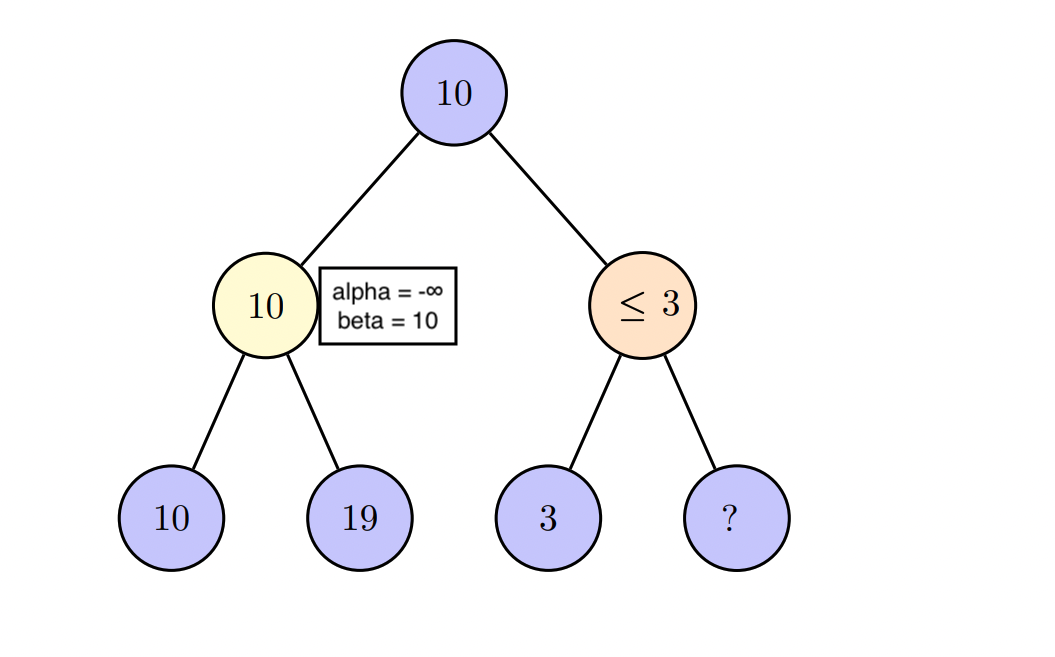
\includegraphics[scale=0.23]{images/pruning_tree3.png}
    \caption{Alpha-beta pruning}
    \label{figure:prunning3}
\end{figure}

Since beta represents the best value for the minimizing-player at a particular position at the tree and the current node is a minimizing node, beta has to be updated to 10.

The newly calculated values are then passed on to the parent node and switched, resulting in alpha being 10 and beta  $\infty $. These values are then further passed on to the next child node which in our case is at depth -1. To that end, the alpha beta evaluation has to be repeated equivalently to the prior alpha/beta determination. Leading to alpha maintaining the value 10 and beta being updated to 3.

\begin{figure}[H]
    \centering
    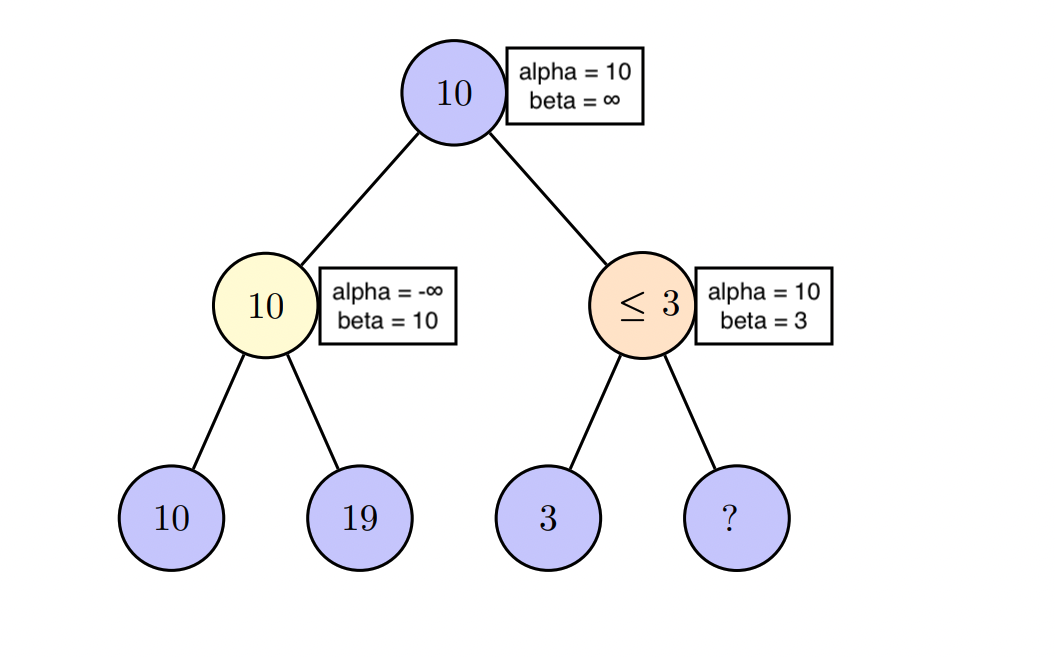
\includegraphics[scale=0.23]{images/pruning_tree4.png}
    \caption{Alpha-beta pruning}
    \label{figure:pruning4}
\end{figure}

Now the alpha and beta values have to be compared to each other and since beta is $\leq \ $ alpha, the node can be pruned.


%%insert pseudocode
%s = state 
%alpha = best value for max at the particular position (path) of the tree
%beta = best value for min at the particular position (path) of the tree

\vspace{1em}
\textbf{Alpha-Beta Variations}

Alpha-beta pruning can be divided into to variations, fail-soft and fail-hard. The difference being that the fail-soft variation updates the alpha and beta value before considering any pruning, whereas the fail-hard prunes before updating any value.
The following subsection shows both algorithms.

\begin{lstlisting}[linewidth=\columnwidth,breaklines=true,mathescape=true,
caption=Fail-hard variation]
def alphaBeta(node, depth, $\alpha$, $\beta$, maximizingPlayer) is
  if depth = 0 or node is a terminal node then
    return the heuristic value of node
  if maximizingPlayer then
    value = -$\infty$
    for each child of node do
        value := max(value, alphaBeta(child, depth - 1, $\alpha$, $\beta$, FALSE))
        
        if value $\ge$ $\beta$ then
            break
        $\alpha$ := max($\alpha$, value)
    return value
  else (* minimizing player *)
    value = +$\infty$
    for each child of node do
        value := min(value, alphaBeta(child, depth - 1, $\alpha$, $\beta$, TRUE))
                                  
        if value $\le$ $\alpha$ then
            break
        $\beta$ := min($\beta$, value)
  return value
\end{lstlisting}

\begin{lstlisting}[linewidth=\columnwidth,breaklines=true,mathescape=true,
caption=Fail-soft variation]
def alphaBeta(node, depth, $\alpha$, $\beta$, maximizingPlayer) is
  if depth = 0 or node is a terminal node then
    return the heuristic value of node
  if maximizingPlayer then
    value = -$\infty$
    for each child of node do
        value := max(value, alphaBeta(child, depth - 1, $\alpha$, $\beta$, FALSE))
        
        $\alpha$ := max($\alpha$, value)
        if value $\ge$ $\beta$ then
            break
    return value
  else (* minimizing player *)
    value = +$\infty$
    for each child of node do
        value := min(value, alphaBeta(child, depth - 1, $\alpha$, $\beta$, TRUE))
                                  
        $\beta$ := min($\beta$, value)
        if value $\le$ $\alpha$ then
            break
  return value
\end{lstlisting}


\begin{lstlisting}[style=ts,linewidth=\columnwidth,breaklines=true,caption=Alpha-Beta Connect-4 source-code]
function alphaBeta(state: State, depth = Infinity): Move | undefined {
	const player = state.player;

    function checkIsTerminal(state: State, currentDepth: number): boolean {
		return currentDepth > depth || state.utility !== 0 || state.moves.length === 0;
	}
	
	function evalFn(state: State): number {
		return player === Cell.PLAYER ? state.utility : -state.utility;
	}
	
	function maximizer(state: State, depth: number, alpha: number, beta: number): number {
		if (checkIsTerminal(state, depth)) return evalFn(state);

		let best = -Infinity;
		const { board } = state;

		for (const move of getActions(state)) {
			const [row, col] = move;

			best = Math.max(best, minimizer(result(state, move), depth + 1, alpha, beta));
			board[row][col] = Cell.EMPTY;

			if (best >= beta) return best;
			alpha = Math.max(alpha, best);
		}

		return best;
	}

	function minimizer(state: State, depth: number, alpha: number, beta: number): number {
		if (checkIsTerminal(state, depth)) return evalFn(state);

		let best = Infinity;
		const { board } = state;

		for (const move of getActions(state)) {
			const [row, col] = move;

			best = Math.min(best, maximizer(result(state, move), depth + 1, alpha, beta));
			board[row][col] = Cell.EMPTY;

			if (best <= alpha) return best;
			beta = Math.min(beta, best);
		}

		return best;
	}
	
    const { board } = state;

	let best = -Infinity;
	let bestMove: Move | undefined = undefined;

	for (const move of getActions(state)) {
		const [row, col] = move;

		const value = minimizer(result(state, move), 1, best, Infinity);
		board[row][col] = Cell.EMPTY;

		if (value > best) {
			best = value;
			bestMove = move;
		}
	}

	return bestMove;
}
\end{lstlisting}

\subsection{Further optimization}
Additionally to the alpha-beta pruning there are other options to improve the algorithm's run time, which can be summarized to ordering heuristics, aspiration search and Killer heuristics. \cite{jonathan1989historyHeuristic}\cite{nasa2018alpha}


\subsubsection{Ordering heuristic}
Ordering heuristic can be used to figure out whether a move is going to potentially cause an alpha beta cutoff.Inner nodes, which are essentially all nodes except the root node or leaf nodes, are ordered accordingly to optimize the algorithm's run time. The best ordering for the inner nodes is logic based and can be calculated. Some techniques include iterative deepening, transposition tables and refutation tables. \cite{jonathan1989historyHeuristic}


\subsubsection{Aspiration search }
This technique narrows down the window in which the search is taking place. To put it another way, the search window is determined by the alpha and beta difference. Meaning that a low difference between these values can lead to a smaller search window which would subsequently result in better search performances. However if the search does not lead to the desired outcome the search window has to be broaden and the search restarted. \cite{jonathan1989historyHeuristic}



\subsubsection{Killer heuristic }
Killer heuristics are based on making use of already existing information. To that end, a node's sub-tree information is appraised and stored for potential use. If a certain node causes a cutoff, this move will be examined first when traversing the tree again. The information is collectively regarded for each depth level. For example, if a node at depth 2 triggers the most cutoffs it is most likely going to cause similar effects the second time the tree is searched.
Researches have proven that even though reordering inner nodes takes up time resources, it still leads to a overall better performance. In general, knowledge based on the application is used to determine more use case specific heuristics. If the information's quality is not sufficient enough implementation will most likely add calculated search evaluations to the evaluation.
Nevertheless would even an imperfect heuristic lead to better results. \cite{jonathan1989historyHeuristic}



%%%%%%%%%%%%%%%%%%%%%%%%%


%%%%%%%%%%%%%%%%%%%%%%%%


%\vspace{1em} 
\section{Related work}
MinMax algorithm is undoubtedly not the first algorithm created for simultaneous move games. Over the past decades there have been multiple adaptations to the problem, which can be summarize into the following three categories.
\cite{branislav2016algorithms}

\subsection{Iterative learning algorithms}
Iterative learning algorithms are based on self-play strategies, which are determined by iterating through the tree.

In 2000 new adaptations for this algorithm were presented,including the no-regret algorithm, which was then applied to One-Card Poker. Additionally a counterfactual regret minimization (CFR) was introduced, which generally speaking finds it's use in games obtaining a larger amount of information. Subsequently CFR was used for Poker AI and resulted in an algorithm efficient enough for solving Head up limit Texan Hold'em. \cite{bowling2015hold'em_poker}

A variation of this technique called iterative deepening can be used for MinMax optimization. Hereby the search tree is traversed ply after ply, which is a half move. After each move the depth value gets incremented. Also every iteration has a certain amount of time allocated to it in which it should execute the iteration. If the time runs out and the process has not finished yet, it gets terminated and has to be executed again.
The algorithms main goal is to increase the probability of searching the best move from the root onwards. Meaning that the best path is already picked at the beginning. (often used for depth first search algorithms)


\subsection{Exact backward induction algorithms}
Exact backward induction algorithms are based on a recursive iteration of the tree, which obtains information based on a node's child value. This technique is mostly used in sequential games but can be altered in order to suit  simultaneous move games.


\subsection{Approximative sampling algorithms}
Approximate sampling algorithms generate samples according to a given distribution. These examples can be used to further predict the probability of potential moves. \cite{spyridon2005sampling-approximation}
\\
A common algorithm that uses this technique is called Monte Carlo Tree Search(MCTS), which is utilized in extensive-form games. \cite{branislav2016algorithms} These make use of a certain tree search which also considers the amount of time needed to actually choose a move.
The MCTS's functionality was proven by the success of the game Go and was later on adapted with UCB (upper confidence bounds) which was then used in the game Tron. \cite{spyridon2010uctAgentTron}


%-> "black-box" -> creates samples  %https://www.math.uwaterloo.ca/~cswamy/papers/multistagefnl.



\vspace{1em}
\section{Conclusion}
In this paper, the main principles of the MinMax algorithms were analysed. We did not only look at the function itself but also into optimization techniques such as alpha/beta pruning and further techniques which included ordering heuristics, aspiration search and killer heuristics. Additionally we looked into related algorithms and there use cases.


%%%%%%%%%%%%%%%%%%%%%%%%%%%%%%%%%%%%
\clearpage
%%%%%%%%%%%%%%%%%%%%%%%%%%%%%%%%%%%%

%%%%%%%%%%%%%%%%%%%%%
\bibliographystyle{IEEEtran}
\bibliography{quellen}
%%%%%%%%%%%%%%%%%%%%%

\end{document}
